
\subsection{4-2-4 Econder} 
\label{sec:tlr-auto4} 

\ref{sec:datasets-auto4} 
%======== (3D) L1 x L2 x patSuccF =========
%TODO treat as main plot of the work 
%TODO (add plane of best BAL) 
\begin{figure}[t]
  \centering
  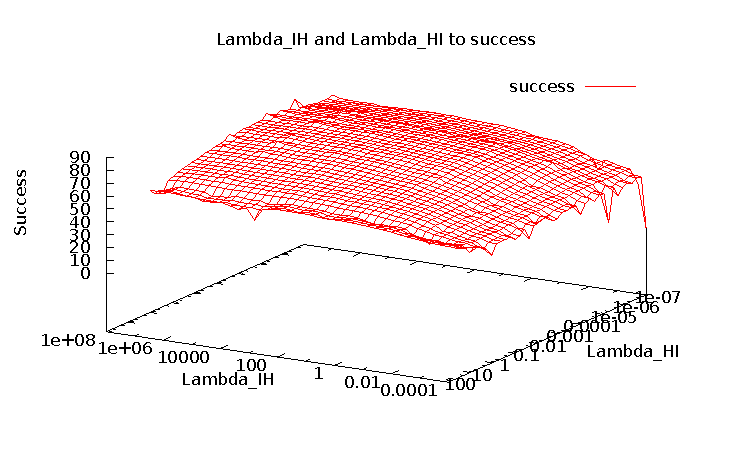
\includegraphics[width=0.8\textwidth]{img/success_to_lambdas.pdf}    
  \caption{Encoder 4-2-4: Performance of the TLR model with $\sigma = 2.3$ and $\mu = 0.0$.}
  \label{fig:results-two-lambdas-auto4-success}
\end{figure}

%======== (3D) L1 x L2 x epochs =========
%TODO logaritmic scale of epochs + label 
\begin{figure}[t]
  \centering
  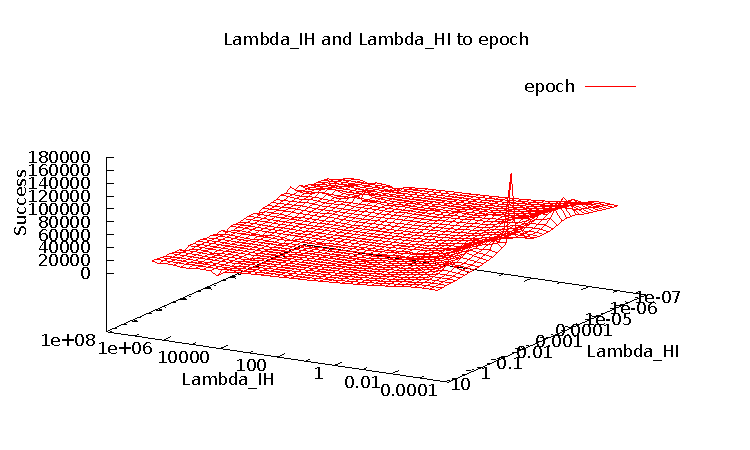
\includegraphics[width=0.8\textwidth]{img/epoch_to_lambdas.pdf}    
  \caption{Encoder 4-2-4: Convergence time of the TLR with $\sigma = 2.3$ and $\mu = 0.0$.}
  \label{fig:results-two-lambdas-auto4-epoch}
\end{figure}

%======== (2D) best TLR on ALL_SUCC x epoch (std-dev) ==========
% TODO bitSucc, patSucc, F,B + std_dev 
\begin{figure}[t]
  \centering
  \includegraphics[width=0.8\textwidth]{../bal/data/stats/test/epoch_to_success.pdf}    
  \caption{Encoder 4-2-4: Epoch to success of the best Two learning rate setting for $\lambda_v = $ and $\lambda_h=$ (TODO values).}
  \label{fig:results-two-lambdas-auto4-s2e} 
\end{figure}
